%&tex
\documentclass{standalone}

\usepackage[dvipsnames]{xcolor}

\usepackage{tikz}
\usetikzlibrary{positioning,shadows}
\usetikzlibrary{arrows,chains,positioning,scopes,shapes.geometric,shapes.misc,shadows,decorations.markings}


\begin{document}

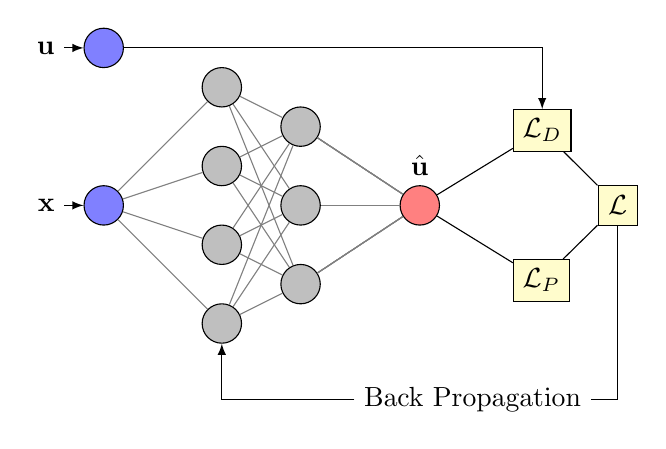
\begin{tikzpicture}

	% \draw[help lines, step=1cm,gray!20] (0,0) grid (10,5);

    % input layer node
    \node[draw,
    circle,
    minimum size = 0.5cm,
	fill=blue!50] (X) at (0,1) {};

    % input layer node
    \node[draw,
    circle,
    minimum size = 0.5cm,
	fill=blue!50] (U) at (0,3) {};

	% hidden layer nodes
	\foreach \i in {1,...,4}
	{
		\node[draw,
		circle,
		minimum size = 0.5cm,
		fill=gray!50] (HL_1-\i) at (1.5, \i-1.5) {};
	}

	\foreach \i in {1,...,3}
	{
		\node[draw,
		circle,
		minimum size = 0.5cm,
		fill=gray!50] (HL_2-\i) at (2.5, \i-1) {};
	}

	\node[](BackPropagation) [below right = 0.5cm and 1.5cm of HL_1-1] {Back Propagation};

	% output layer
	\node[draw,
	circle,
	minimum size = 0.5cm,
    label = $\hat{\mathbf{u}}$,
	fill=red!50] (T) [right = 1.0cm of HL_2-2] {};

	% data loss loss function
	\node[draw,
	rectangle,
	minimum width = 0.5cm,
	minimum height = 0.5cm,
    fill=yellow!20] (LD) [above right = 0.5cm and 1cm of T] {$\mathcal{L}_D$};

	% physics loss function
	\node[draw,
	rectangle,
	minimum width = 0.5cm,
	minimum height = 0.5cm,
    fill=yellow!20] (LP) [below right = 0.5cm and 1cm of T] {$\mathcal{L}_P$};

	% total loss function
	\node[draw,
	rectangle,
	minimum width = 0.5cm,
	minimum height = 0.5cm,
    fill=yellow!20] (L) [right = 2cm of T] {$\mathcal{L}$};

	% drawing connectors
	\foreach \j in {1,...,4}
	{
		\draw[color=black!50] (X) -- (HL_1-\j);
	}
	\foreach \i in {1,...,4}
	{
		\foreach \j in {1,...,3}
		{
			\draw[color=black!50] (HL_1-\i) -- (HL_2-\j);
			\draw[color=black!50] (T) -- (HL_2-\j);
		}
	}

    \draw[color=black] (T) -- (LP);
    \draw[color=black] (T) -- (LD);
    \draw[color=black] (LP) -- (L);
    \draw[color=black] (LD) -- (L);

    \draw[color=black] (L) |- (BackPropagation.east);
    \draw[-latex,color=black] (BackPropagation.west) -| (HL_1-1.south);
    \draw[-latex,color=black] (U) -| (LD.north);

    \draw[latex-,color=black] (X) -- ++(-0.5,0) node[left]{$\mathbf{x}$};
    \draw[latex-,color=black] (U) -- ++(-0.5,0) node[left]{$\mathbf{u}$};

	% % \draw[-latex,color=black] (T) -- (LD);
	% \draw[-latex,color=gray,opacity=0.2] (T) -- (LD);
	% \draw[-latex,color=gray,opacity=0.2, shorten >= 5mm] (Tinp) -| (LD);
	% % \draw[-latex,color=black, shorten >= 5mm] (Tinp) -| (LD);
	% \draw[latex-,color=black, shorten <=1mm] (X) -- ++(-1,0) node[left]{$x$};
	% \draw[latex-,color=black, shorten <=1mm] (Y) -- ++(-1,0) node[left]{$y$};
	% % \draw[latex-,color=black, shorten <=1mm] (Tinp) -- ++(-1,0) node[left]{$T$};
	% \draw[latex-,color=gray,opacity=0.2, shorten <=1mm] (Tinp) -- ++(-1,0) node[left,color=gray,opacity=0.2]{$T$};
	% % \draw[-latex,color=black, shorten >=1mm] (LD.east) -- ++(1,0) node[right]{$L_D$};
	% \draw[-latex,color=gray,opacity=0.2, shorten >=1mm] (LD.east) -- ++(1,0) node[right,color=gray,opacity=0.2]{$L_D$};
	%
	% \node[](Pnt1) [below = 0.5cm of HL_2-1]{};
	%
	% % \draw[-latex,color=black] (BackPropagation.west) -| (Pnt1.center);
	% % \draw[color=black]  (LD.south) |- (BackPropagation.east);
	% % \draw[color=black] (Pnt1.center) -| ++(1.75,0.2) ;
	% % \draw[color=black] (Pnt1.center) -| ++(-1.75,0.2) ;
	% \draw[-latex,color=gray,opacity=0.2] (BackPropagation.west) -| (Pnt1.center);
	% \draw[color=gray,opacity=0.2]  (LD.south) |- (BackPropagation.east);
	% \draw[color=gray,opacity=0.2] (Pnt1.center) -| ++(1.75,0.2) ;
	% \draw[color=gray,opacity=0.2] (Pnt1.center) -| ++(-1.75,0.2) ;

\end{tikzpicture}

\end{document}
